\section{Introduction}
Since its original proposal \citep{Cox1972}, Cox proportional hazards regression has become the most common regression approach for analyzing survival data.  Cox regression utilizes a partial likelihood construction under an assumption of proportional hazards to estimate the regression coefficients without having to specify the underlying baseline hazard.  The ability to avoid choosing a specific parametric distribution for the survival time is very attractive, as time-to-event data is often poorly described by fully parametric models, but this semiparametric approach comes at a cost.

The Cox regression approach can estimate relative risks, but without estimating the baseline hazard, it cannot make any predictions concerning the absolute failure time for any given individual.  This poses a challenge to assessing the predictive accuracy of a given Cox regression model.  The challenge is particularly relevant for penalized Cox regression \citep{Tibshirani1997,Fan2002}, as the assessment of predictive accuracy via cross-validation is the standard method for selecting the regularization parameter and deciding upon a model.

Standard cross-validation involves of dividing the data into $K$ folds, then fitting the model on $K-1$ of those folds (the training set) and assessing prediction accuracy on the remaining fold (the testing set).  For Cox regression, the estimated coefficients allow us to quantify the risk for each subject in the training set relative to other members of the training set, but it is not obvious how to use those estimates to quantify the model's accuracy in the testing set.

One approach is to simply calculate the partial likelihood based on the observations in the test set as a measure for the model's predictive accuracy.  In doing so, we calculate the risk for each member of the test set relative to other members of the test set.  One drawback to this approach is that it becomes unstable when the size of the the test set is small.  In particular, it cannot be applied to leave-one-out cross-validation (LOOCV), as we must have at least two observations in the test set to compare their risk relative to each other.

%In this paper, we briefly review existing approaches for meeting this challenge, then propose two new methods for carrying out cross-validation in Cox regression models.

%As a semi-parametric model, Cox regression only gives estimations of the $\beta$ coefficients, without estimating the baseline hazard. Hence the interpretation of the Cox model is only valid in a relative sense.

% NOTE: I don't know that we need this paragraph; cross-validation is pretty common.
%One common approach for selecting the tuning parameter $\lambda$ for linear regression and logistic regression is via the K-fold cross validation. The data set would be split into K folds. One fold would be treated as the test set and the other K - 1 folds as the training set. The model would first be built on the training set, then fitted to the test set to obtain cross validation error (CVE).  CVE would be calculated for each candidate $\lambda$, then the one that minimizes cross validated error would be selected.

To overcome this drawback, an alternative approach was proposed by \citet{Verweij1993}.  Their approach, which we describe in detail in Section~\ref{Sec:cox-cv-existing}, stabilizes the cross-validated log likelihood, enabling its use even when the number of subjects in each fold is small.  This approach has been widely used and is implemented in R packages such as {\tt glmnet} \citep{glmnet}.  Although this approach fixes the stability issue, we demonstrate here that in practice, it tends to behave conservatively in terms of model selection.

In this paper, we propose two alternative ways to carry out cross validation for Cox regression. Instead of cross-validating over partial likelihood, we propose cross validation over either the linear predictors of the regression model or over the deviance residuals \citep{Therneau1990}. Through simulation studies, we compare these proposed methods with existing cross-validation approaches for LASSO penalized Cox regression in both low- and high-dimensional settings.  We find that all cross validation approaches tend to be conservative, but that the linear predictor approach offers the best combination of performance and stability, and we recommend using it for regularization parameter selection in penalized Cox models.  We conclude by applying both proposed and existing approaches to two high dimensional data sets from real studies with time-to-event outcomes.

\section{Methods}

In the Cox model, the hazard function for subject $i$ is given by 
\begin{equation}
  h_{i}(t) = h_{0}(t) \exp( X_{i}^{T} \beta),
\end{equation} 
where $h_{0}$ is the baseline hazard and $e^{X_i^{T} \beta}$ is the risk for a subject with covariates $X_i$ relative to that baseline.  The estimation of the coefficients is obtained by maximizing a partial likelihood.  Letting $t_i$ denote the time on study for subject $i$ and $\delta_{i}$ indicate whether or not an event is observed for subject $i$, each subject's individual contribution to that partial likelihood is
\begin{equation}
  l_{i}(\beta) = \left \{\frac{\exp ( X_{i}^{T} \beta)}{\sum_{ k \in R(t_{i})}\exp ( X_{k}^{T} \beta)}\right \}^{\delta_{i}},
\end{equation}
where $R(t_{i})$ denotes the set of subjects at risk at time $t_{i}$.  The partial likelihood for the entire sample of $n$ subjects is then given by:
\begin{equation}
  L(\beta) =\prod_{i = 1}^{n} l_{i}(\beta).
\end{equation}

Cox regression can be extended by introducing a penalty into the partial likelihood.  In penalized Cox regression, $\beta$ coefficient estimates are obtained by minimizing the objective function
\begin{equation}
  Q(\beta) = - \frac{1}{n} \log L(\beta) + P_{\lambda}(\beta),
\end{equation}
where $P_{\lambda}(\beta)$ is a penalty function that depends on a regularization parameter $\lam$. In this paper, we focus upon the LASSO penalty $P_{\lambda}(\beta) = \lambda (\sum_{j} |\beta_{j}|)$, although the methods we propose can be used with any penalty (indeed, can also be used for model selection in unpenalized Cox regression).  LASSO cox regression is particularly useful for high dimensional data where the number of covariates p $\gg$ n; for example, in the prediction of cancer patients' overall survival based on genome-wide expression measurements.

Selecting $\lambda$ is critical to LASSO estimation. LASSO estimates are sparse, in the sense that some coefficients are estimated to be exactly zero, thereby carrying out automatic variable selection along the solution path. At large values of $\lambda$, most or all of the coefficients are 0, but as $\lam$ decreases, more covariates are selected into the model. If $\lam$ is too large or too small, the model's predictive accuracy suffers.

\subsection{Cross Validated Likelihood} 
\label{Sec:cox-cv-existing}

Suppose a data set of n observations is split into K folds and the ith fold is left out, then a partial likelihood can be built over the K -1 folds and yields maximum likelihood estimates of the coefficients, denoted by $\hat{\beta}_{-i}$. An intuitive way to carry out cross validation is to use the partial likelihood on the test data as the cross validated error: \begin{equation}cvl = \sum_{i=1}^{K} l_{i}(\hat{\beta}_{-i})\end{equation} This is implemented in the $\tt{glmnet}$ package as the $\tt{ungrouped}$ option. We refer to this definition as standard cross-validated partial likelihood.

An alternative way to calculate cross-validated log likelihood was proposed by Verweij and Van Houwelingen. They defined cross-validated log likelihood of leaving the ith fold out to be \begin{equation}cvl = \sum_{i=1}^{K} \{l(\hat{\beta}_{-i}) - l_{-i}(\hat{\beta}_{-i})\}. \end{equation} When the ith fold is left out, $l(\hat{\beta}_{-i})$ is the log partial likelihood evaluated at $\hat{\beta}_{-i}$ with all k folds of observations. $l_{-i}(\hat{\beta}_{-i})$ is the log partial likelihood evaluated at $\hat{\beta}_{-i}$ with observations from the other K-1 folds. We refer to this definition as Verweij and Van Houwelingen's cross-validated partial likelihood. This is implemented in the $\tt{glmnet}$ package as the default $\tt{grouped}$ option.

\par The upper panels in Figure 2 illustrates the ideas of the two methods. Through substraction, Verweij and Van Houwelingen's approach allows measuring individual observation's contribution to the partial likelihood, so that leave-one-out cross-validation is feasible. Since only the left-out fold would be used to construct the partial likelihood, the standard CVL is unstable in practice when there are only very few observations in some folder. 

  \subsection{Cross Validated Linear Predictors}

Besides cross validating over the partial likelihood, an alternative approach is to cross validate over the linear predictors. In the first step, the ith fold would be left out and the other K-1 folds would be used as the training set to get the estimates $\hat{\beta}_{-i}$. Then, the cross-validated linear predictors would be calculated based on the observations in the test set:  \begin{equation}\hat{\eta}_{-i} = X_{i}\hat{\beta}_{-i}.\end{equation} After repeating this for all K folds, a whole set of linear predictors  $\hat{\eta}_{-} = ( \hat{\eta}_{-1},  \hat{\eta}_{-2} , ...  \hat{\eta}_{-K})$ can be obtained. A partial likelihood can be built over this set of linear predictors: \begin{equation} L(\hat{\eta}_{-}) = \prod_{j=1}^{m} \frac{exp (\hat{\eta}_{-j})}{\sum_{ k \in R(t_{j})}exp (\hat{\eta}_{-k})}\end{equation}.

Cross-validated error is defined as the log of $L(\hat{\eta}_{-})$. This idea of cross validating over linear predictors is implemented in the package \texttt{ncvreg} \citep{ncvreg}. For all the approaches introduced so far, they are all equivalent to each other in linear regressions. But since they are building over different baselines, they are different in cox regression.

  % \begin{figure}[h]
    %\centering
    %\begin{minipage}[b]{0.45\textwidth}
      %\centering
	%	  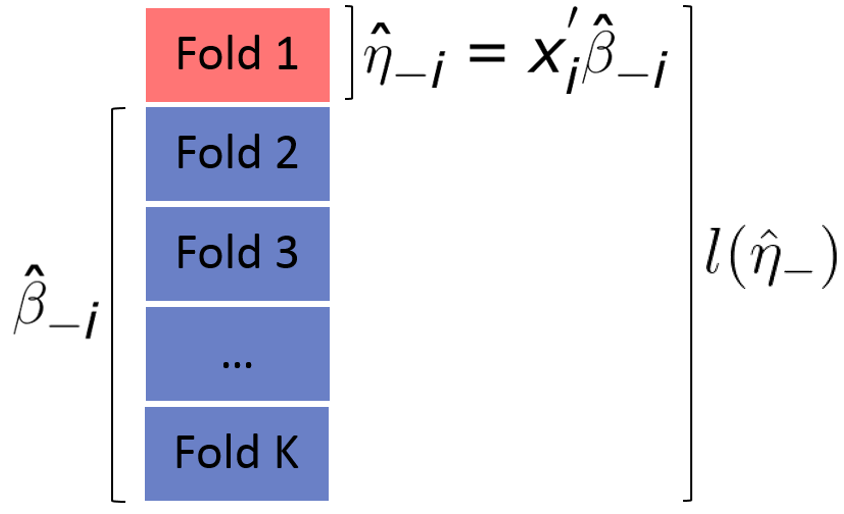
\includegraphics[height= 3.9cm ]{./figures/03.png}
      %\caption{CV Linear Predictors}
     %\end{minipage}
     %\begin{minipage}[b]{0.45\textwidth}
      %\centering
%		  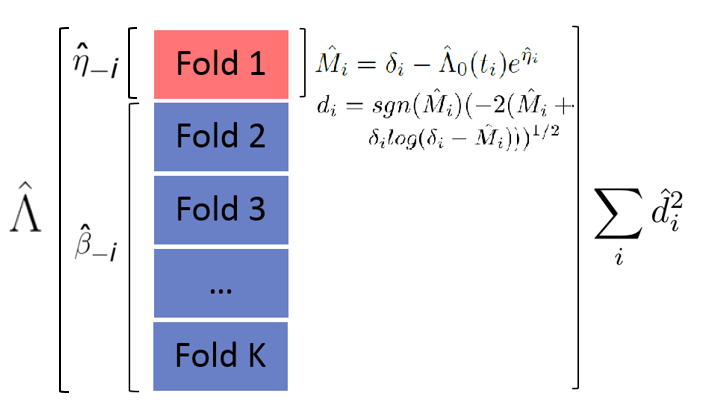
\includegraphics[height= 4.1cm ]{./figures/04_2.png}
    %  \caption{CV Deviance Residuals}
     % \end{minipage}	
  % \end{figure}	
    
  \subsection{Cross Validated Deviance Residuals}
  %Need to update this section with the new baseline estimation method%
The fundamental challenge of conducting cross validation for cox regression is that the baseline hazard is not estimated from the model. Hence we proposed our second approach which involves estimating the actual baseline hazard $\hat{\Lambda}_{0}$. The sum of squares of Martingale residuals is a natural candidate for evaluating the model performance using baseline hazard. Martingale residuals and its normalized form, deviance residuals, were first proposed by \citep{Therneau1990} for Cox regression model diagnostics. 

To estimate the baseline hazard, a set of linear predictors $\hat{\eta}_{-} = ( \hat{\eta}_{-1},  \hat{\eta}_{-2} , ...  \hat{\eta}_{-K})$ would be obtained in the same way as the cross validated linear predictor approach. $\hat{\eta}_{-i}$ is computed based on $\hat{\beta}_{-i}$s estimated from the training set and observations from the ith test set. With $\hat{\eta}_{-}$, a baseline hazard $\hat{\Lambda}_{0}$ can be estimated via Kalbfleisch and Prentice's method \citep{Kalbfleisch2011}. Then for each observations, the Martingale Residual can be calculated: \begin{equation}\hat{M_{i}} = \delta_{i} -\hat{\Lambda}_{0}(t_{i})e^{\hat{\eta}_{i}},\end{equation} where $\delta_{j}$ is the status of the jth observation and $t_{j}$ is the time component of the jth observation. The deviance residual can be calcualted from the Martingale Residuals: \begin{equation} d_{i} = sgn(\hat{M}_{i})(-2(\hat{M}_{i} + \delta_{i}log(\delta_{i} - \hat{M}_{i})))^{1/2}\end{equation} The sum of squares of the deviance residuals, $\sum_{i}\hat{d}_{i}^2$, would be used as the cross validated error. An illustration of this method is drawn in the bottom right panel of Figure 1.

As an alternative, the baseline hazard can also be estimated only based on the training set, leaving the test set as out-of-sample observations for calculating the residuals. There are two major issues with this approach. First, it would be common to run into situations where events in the test set occurred after the last event occurred in the baseline, where the survival function dropped to 0. Unless those observations are treated as censored, this approach would not work. Second, there would be an extra numeric challenge for deviance residuals. Since the baseline hazard function $\hat{\Lambda}_{0}$ is a step function from 0, the cumulative hazard at the first time point from 0 is always 0. Since deviance residual contains a term $log(\delta_{i} - \hat{M}_{i})$, where $\delta_{i} - \hat{M}_{i} = \hat{\Lambda}_{0}$, this term would be negative infinity for the first time point and lead to a numeric issue for whichever fold that contains the first time point. Hence extra smoothing for the step function would be needed for this approach to work.

\begin{figure}
    \centering
		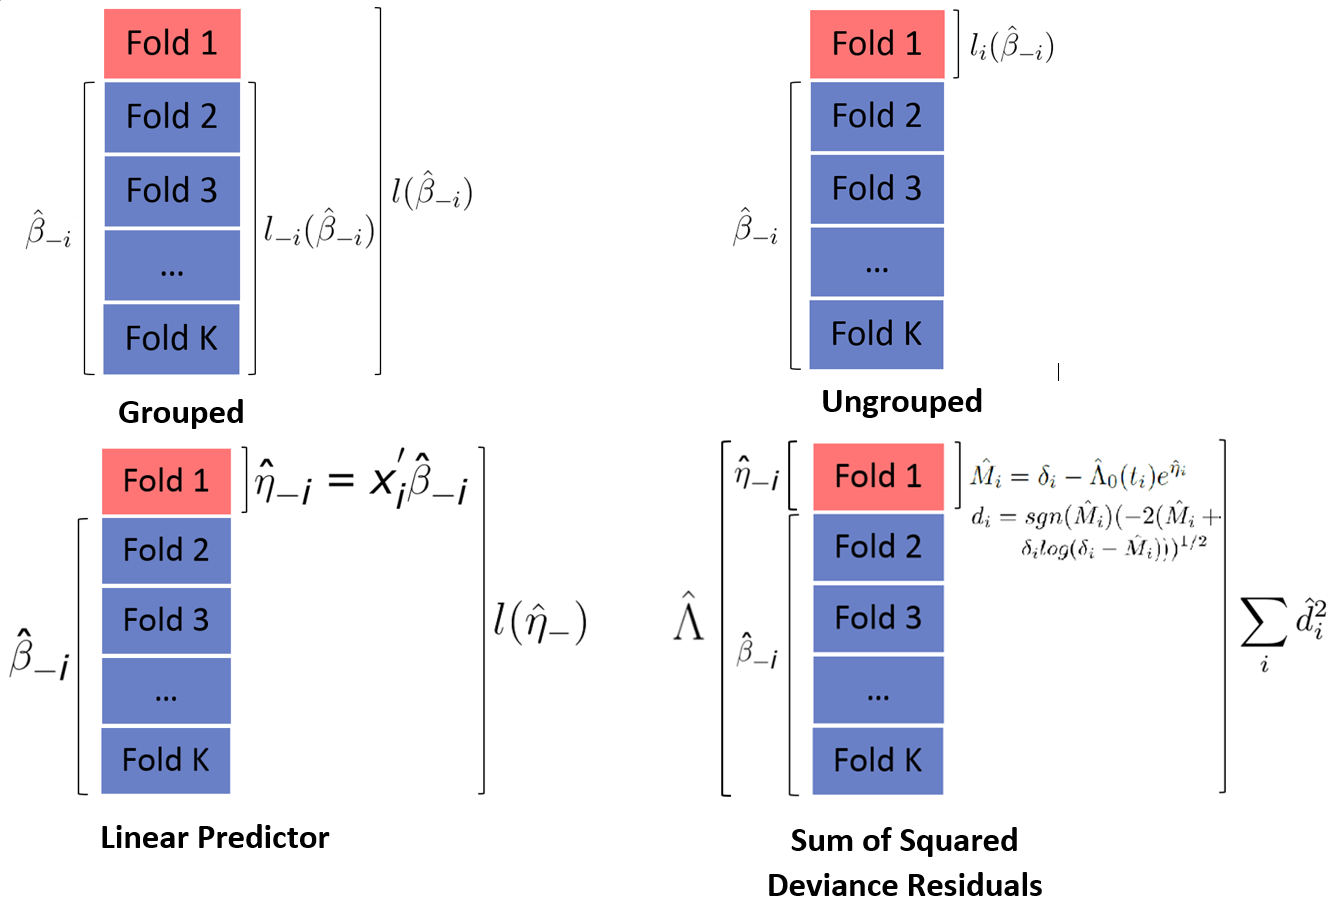
\includegraphics[height= 9cm ]{./figures/figure_1.png}
		%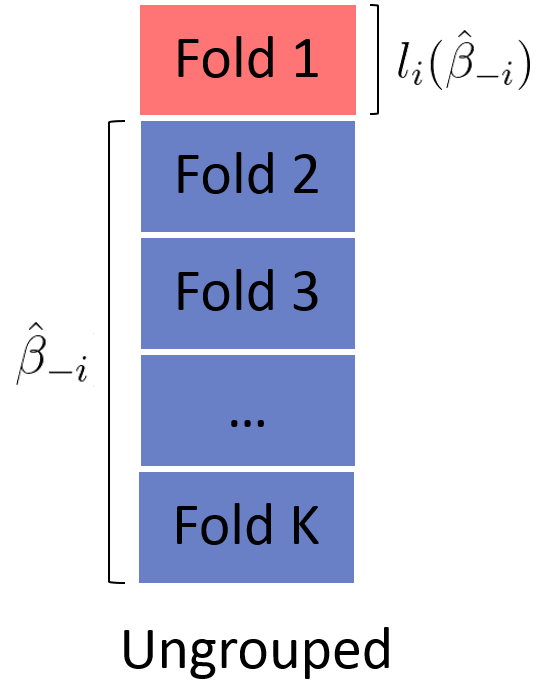
\includegraphics[height= 4cm ]{./figures/02_2.png}
    \caption{Illustration of K-fold Cross Validation Methods for Cox Regression}
\end{figure}	

\note{tranpose sign in figure 1 is corrected}

\section{Simulation Studies}

  Simulation studies were conducted to compare how those methods behave relative to each other. We generated data with pre-specified baseline hazard, covariate matrix X, coefficient $\beta$ and censoring mechanism. Both low dimensional and high dimensional scenarios were examined. All cross-validation methods mentioned in Section 2 were applied to the data to select the tuning parameter $\lambda$ and produce $\hat{\beta}$ estimates. %Cross-validation were also compared to model selection criteria AIC and BIC.
  
 The entries in the covariate matrix $X_{n \times p}$ were independently generated from $Normal(0, 1)$. True coefficients $\beta$ were assumed to have sparsity: $\beta_{p\times 1} = (\beta_{1},\beta_{2}, ..., \beta_{j}, 0, ..., 0)^{T}$. The covariate matrix $X_{n \times p}$ was centered before it was used to generate outcomes. Survival times were generated from exponential distribution $h(t) = h_{0} exp(X\beta)$, conditioned on covariates. Censoring status were generated based on binomial distribution. All simulations were implemented in R \citep{R}.
  
  Suppose $\hat{\beta}$ is the coefficients estimated by a fitted cox model. We quantify the predictive accuracy by measuring the distance between the fitted model and the true model by mean squared error MSE $= E(\hat{\beta} - \beta)^2$. For each generated data set, the $\lambda$ that has the minimal MSE is chosen as the optimal $\lambda$. Then the $\lambda$s that selected by the cross validation or information criteria would be compared to this optimal $\lambda$. If the $\lambda$ chosen by cross validation is smaller than the optimal $\lambda$, then the cross validation method would be considered liberal. If the $\lambda$ chosen by cross validation is larger than the optimal $\lambda$, then the cross validation method would be considered conservative. 
     
    \subsection {Simulations Comparing Cross-validation Approaches}
  %need to change figures to include the new cross-validated deviance residuals
   The simulation experiments were first conducted when the signal in the data was varied. In each simulated data set, there are n = 100 observations and p = 1000 covariates. 10$\%$ of the observations were censored. 10-fold cross-validation was implemented for all four methods. Number of non-zero $\beta$s was 20. The signal in the data set was varied by varying the magnitude of the $\beta$s from 0.50 to 1.50. For each scenario, 200 replications were used.
   
\begin{figure}[h]
    \centering
		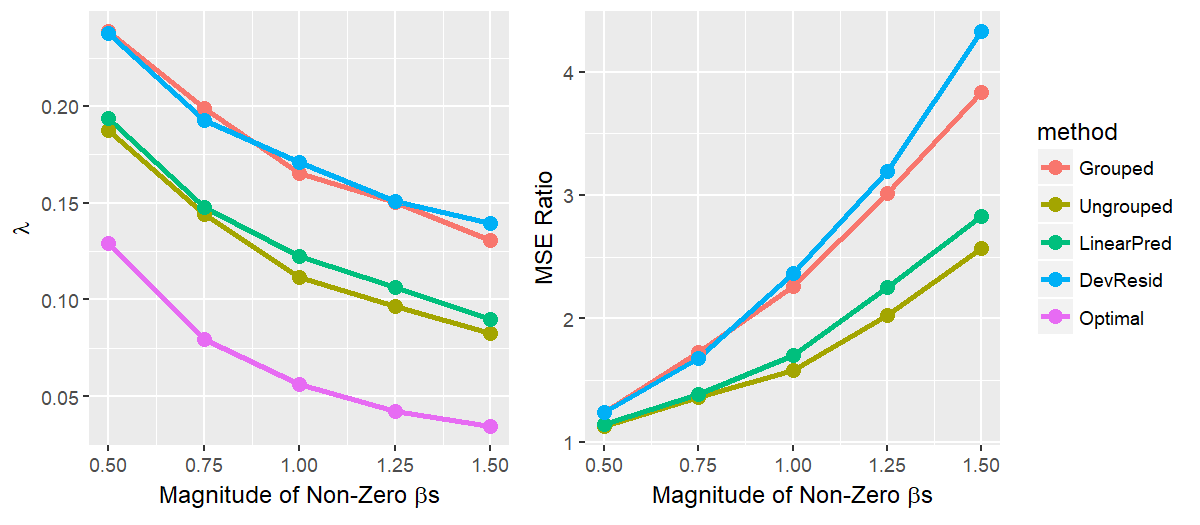
\includegraphics[height= 7cm ]{./figures/figure_2.png}
    \caption{Simulation Studies Comparing 4 CV methods in terms of $\lambda$ and MSE ratio. n = 200, p = 1000, 10$\%$ censoring.}
\end{figure}	

\par Results of this simulation were illustrated in Figure 2.  The x axis of the plots are the magnitude of the non-zero $\beta$ coefficients. The left panel compares the $\lambda$ selected by different methods. Verweij and Van Houwelingen's cross-validated partial likelihood approach, which is currently most widely used approach, consistently selects $\lambda$s that are greater than the optimal one.  Greater $\lambda$ leads to greater penalties and fewer non-zero variables, hence Verweij and Van Houwelingen's approach is conservative in terms of selecting variables. While the proposed cross-validated Deviance residual has very close performance as Verweij and Van Houwelingen's approach, the standard cross-validated log likelihood and the cross-validated linear predictor were more liberal than the other two methods. In general, all four methods tends to act conservatively and selects smaller models. 

\par The right panel compares the MSE ratios of the model selected. The MSEs of the cross-validation selected models are compared with the MSE of the model given by the optimal $\lambda$. The y-axis represents the ratio of the two. The standard method has the smallest MSE ratio. The linear predictor approach's performance is also very close the standard approach. Both Verweij and Van Houwelingen's approach and the proposed deviance residual approach yield models that have greater MSE, hence are not recommended for use in practice.
 
\begin{table}[h]
\small
\centering
\caption{Simulations Comparing all four Cross-Validation methods, Varying n and p}
\begin{tabular}{llllllllllllllll}
\hline\\[-0.75em]
       & \multicolumn{3}{l}{n = 100, p = 20} &  & \multicolumn{3}{l}{n = 100, p = 100} &  & \multicolumn{3}{l}{n = 500, p = 10000} &  & \multicolumn{3}{l}{n = 250, p = 10000} \\
       & \multicolumn{3}{l}{$\#$of non-zero = 10} &  & \multicolumn{3}{l}{$\#$of non-zero = 10} &  & \multicolumn{3}{l}{$\#$of non-zero = 20} &  & \multicolumn{3}{l}{$\#$of non-zero = 20} \\ \cline{2-4} \cline{6-8} \cline{10-12} \cline{14-16} 
\hline\\[-0.75em]
       &     &        &MSE       &  &   &       & MSE     &    &    &        & MSE      &  &     &        & MSE      \\
       & $\lambda$ (SD)     & &Ratio       &  & 	$\lambda$ (SD)         & & Ratio     & &	$\lambda$ (SD)         & & Ratio      & &	 $\lambda$ (SD)         & & Ratio      
\\ 
\cline{2-2} \cline{4-4} \cline{6-6} \cline{8-8} \cline{10-10} \cline{12-12} \cline{14-14} \cline{16-16} 
\\[-0.75em]
Optimal &0.016 (0.009)&&/&&0.042 (0.003)&&/&&0.026 (0.001)&&/&&0.026 (0.001)&&/\\          
V $\&$ VH &0.035 (0.007)&&2.597&&0.073 (0.009)&&2.184&&0.053 (0.003)&&5.627&&0.123 (0.036)&&3.931\\
Standard &0.030 (0.009)&&2.246&&0.064 (0.01)&&1.815&&0.040 (0.003)&&3.131&&0.070 (0.016)&&2.560\\
LinearPred &0.034 (0.007)&&2.559&&0.066 (0.008)&&1.880&&0.041 (0.003)&&3.350&&0.074 (0.016)&&2.713\\
DevResid &0.100 (0.009)&&14.005&&0.108 (0.008)&&4.087&&0.076 (0.003)&&9.133&&0.111 (0.028)&&3.767\\ 
\hline
\end{tabular}
\end{table}

\par Simulation studies were also conducted in scenarios with various sample sizes and dimensions. The results are shown in Table 1. While the standard approach yields the smallest MSE and best predictive accuracy, the Linear Predictor and the standard approaches perform closely to each other across all settings. Verweij and Van Houwelingen's approach performs well in low-dimensions or with sufficient samples, while deviance residual approach performs better in high-dimensional settings.

 \subsection {Stability}
  
\par In this section, simulations studies were conducted to address the stability issue of the standard cross-validated likelihood. The standard approach is an intuitive way to carry out cross-validation. It also has the best predictive accuracy based on the simulation results in previous sections. However, one big disadvantage of this approach is that it is unstable when number of observed events in some fold is really small. As is illustrated in Figure 3, when censoring increases or when number of folds increases, the model would fail to converge due to insufficient number of events in the test set. Hence, the standard cross-validated likelihood should not be used when there is no sufficient number of events.

\begin{figure}[h]
    \centering
		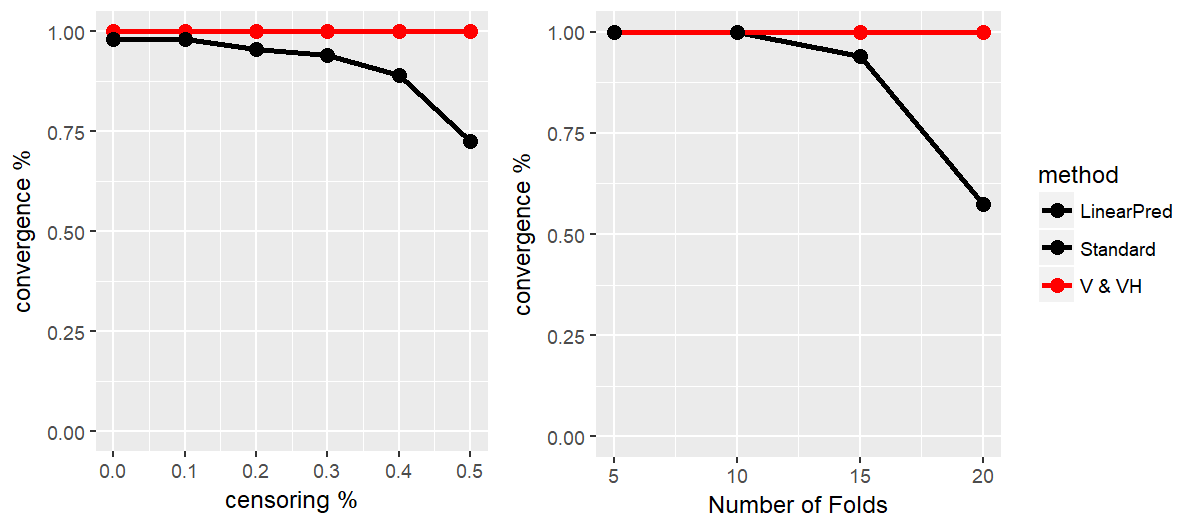
\includegraphics[height= 7cm ]{./figures/figure_3.png}
    \caption{Comparing Stability}
\end{figure}	

    \subsection {Results of Leave-One-Out Cross Validation}
	\par In this section, Leave-One-Out Cross Validation (LOOCV) were studied, in comparison with 10-fold CV. When first introduced, Verweij and Van Houwelingen's cross-validated partial likelihood was proposed so that LOOCV for Cox regression became feasible. It is impossible to carry out LOO cross-validation using the standard approach, because the partial likelihood cannot be built on the one left-out observation. While Verweij and Van Houwelingen's cross-validated partial likelihood solves the stability issue by aggregating more observations together, it is not an efficient way to evaluate the model fit. Simulation studies in Section 3.1 have illustrated that it tends to be conservative in variable selections and selects smaller models in various scenarios. This fact can be even more illustrated via the following simulation studies, where both 10-fold and LOOCV were conducted via Verweij and Van Houwelingen's approach, linear predictor and deviance residual approaches and 10 fold CV was conducted for the standard approach.
	\par As is illustrated in Figure 4, LOOCV selected models that have smaller MSE than 10-fold CV for all three CV approaches. As is shown in left and middle panels, LOOCV based on deviance residuals and Verweij and Van Houwelingen's cross-validated partial likelihood still perform more conservatively than the standard approach. Even if Verweij and Van Houwelingen's approach was proposed to allow LOOCV, the LOOCV based on Verweij and Van Houwelingen's approach does not surpass the 10-fold standard approach. On the other hand, the Linear Predictors also allows LOOCV, and the LOOCV based on Linear Predictors performs better than the standard approach.

    %\par We also compared cross-validation with information criteria AIC and BIC. Simulation studies were conducted in lower dimension and higher dimension respectively. As is illustrated in Figure 7, in lower dimension, AIC tends to perform more liberal and BIC tends to perform more conservative than the optimal $\lambda$. While the cross-validation methods are also conservative, most of them are less conservative than BIC. In terms of MSE, cross-validation methods yield smaller MSE than the information criteria. In higher dimension, both BIC and AIC tend to be more liberal than the optimal $\lambda$ and yield larger MSE.

\begin{figure}[h]
    \centering
		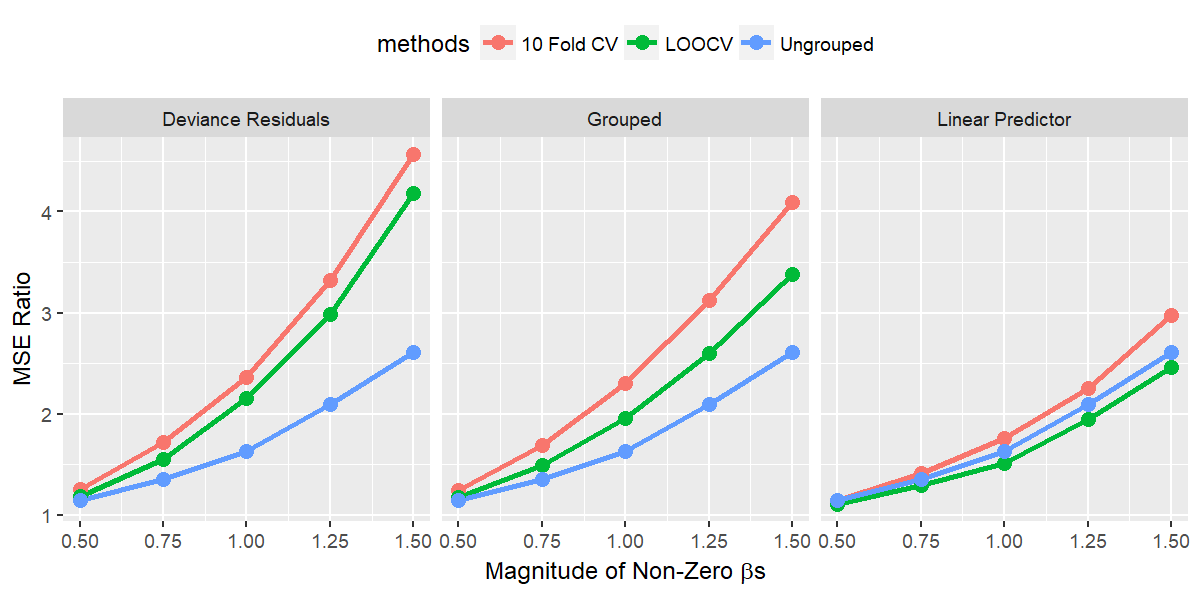
\includegraphics[height= 8cm ]{./figures/figure_4.png}
    \caption{LOOCV}
\end{figure}	

  \subsection {Simulations on Deviance Residuals and Baseline Hazard Estimations}
\par While the Deviance Residual approach has a reasonable performance in scenarios where dimension is high, it tends to act more conservatively than all the other three approaches in general. As is noted by Therneau et al, the sums of squared martingale residuals and deviance residuals do not necessary reflect how good the model fit is \citep{Therneau2000modeling}. The difficulty of estimating the baseline hazard seems to play an important role. A series of simulations were thus designed to study how baseline hazard estimation affects the deviance residuals' performance as a measurement for model fit. 

\par In the following simulation studies, the defined optimal $\lambda$ and the $\lambda$ selected by the Linear Predictor approach were used as benchmarks. Various sample sizes and dimensions were varied. The survival outcomes were generated both from exponential distribution and Weibull distribution. Six different approaches were compared in terms of baseline hazard estimation and their impact on sums of squared deviance residuals. Two non-parametric approaches, Kalbfleisch and Prentices' estimator and Breslow's estimator, were used first for estimating the cumulative hazard baseline \citep{Kalbfleisch2011} \citep{breslow1972}.  As is presented in column 3 and column 5 in Table 2, the sum of squared deviance residuals computed based on both approaches are all very conservative compared to the optimal $\lambda$. Their performance is extremely bad when n is large and p is small. 

\par Since both of the non-parameteric estimations seemed to perform well at early time points but poorly later, a weighted approach was then applied to emphasize earlier time points. Weights are assigned proportional to number of subjects at risk, making earlier time points weighted more than later time points. Results of these two approahces are presented in column 4 and 6 in Table 2. The attempt to improve the non-parameteric estimations via weighting does not seem to improve the selection too much. 

\par In the next step,  the non-parametric baseline hazard estimation was replaced by the exact baseline hazard that was used to generate the outcome. Results were listed in the seventh column in Table 2. When the baseline was known, the performance of sum of squared deviance residuals actually performed really close to the optimal $\lambda$. This simulation suggests that when the baseline hazard was accurately estimated, then the sum of squared deviance residuals gave really good measures for the model fit.

\par In the last step, we replaced the non-parametric baseline hazard estimation with a parametric approach, where we assume the baseline hazard to follow an exponential distribution. We derived the estimation for baseline hazard by maximum likelihood approach conditioned on covariates: $\hat{\lambda}_{0} = \frac{\sum d_{i}}{\sum t_{i}e^{\eta_{i}}}$. The results are listed in the eighth column in Table 2. When this estimation was used for data that were generated from exponential distribution, its performance was as well as when the exact baseline was specified. When it was fitted to data that were generated from the Weibull distribution, that is when the model is misspecified, then its performance was even worse than the non-parametric approaches.

\par Hence, getting accurate estimation of the baseline hazard is crucial to whether or not the sum of squared deviance residuals can be a good measurement for model fit.

\begin{table}[h]
	\small
	\caption{Average of Selected $\lambda$ with Different Baseline Estimation for Deviance Residuals}
	\centering
	\begin{tabular}{lllllllll}
	\hline
	\\[-0.75em]
    & Optimal & Linear Pred & KP & KP & Breslow & Breslow & Exact & Exp\\ 
    &  & & & weighted & & weighted & & \\ \cline{2 - 9} 
\textbf{True Baseline: $Exponential(1)$} &&&&&&&&\\
n = 100, p = 10, non-zero $\beta$: 2 & 0.0461 & 0.0665 & 0.1986 & 0.1970 & 0.1908 & 0.1975 & 0.0540 & 0.0539 \\
n = 100, p = 100, non-zero $\beta$: 20 &0.0555 & 0.1841 & 0.2359 & 0.2201 & 0.2146 & 0.2244 & 0.0805 & 0.0985 \\
n = 100, p = 1000, non-zero $\beta$: 20 & 0.0268 & 0.0505 & 0.0948 & 0.0798 & 0.0867 & 0.0809 & 0.0288 & 0.0270 \\
\textbf{True Baseline:} $Weibull$ &&&&&&&& \\
 n = 100, p = 10, non-zero $\beta$: 2 & 0.0476 & 0.0710 & 0.2004 & 0.1969 & 0.1907 & 0.1907 & N/A & 0.2330 \\ 
\hline
\end{tabular}
\end{table}

\section{Application to Real Data}

\par In this section, we compared the performances of those cross validation methods when they are applied to data from real studies. The first data set is collected from a study on ovariance cancer from The Cancer Genome Atlas. The second dataset is a study on lung cancer \citep{shedden2008gene}. The outcomes of both data sets are patients' overall survival time.

\par In the ovarian cancer data set, there are 460 patients and 236 events . About 40$\%$ of the observations are censored. The covariate matrix records whether or not there is mutation at certain gene location and has dimension of 12376. Three clinical variables, age, gender and residuals, which were known to have large impact on survival were adjusted in the analysis. That is to say, the clinical covariates were first fitted into regular cox regression and only linear predictors were kept so that the selection for the penalty term would not affect the estimation of those clinical variables. Cross-validation was used for the selection of the penalty term, which affects the selection of gene mutations. The results are illustrated in Table 3. 

\par In the lung cancer data set , researchers collected gene expression data for 22283 genes. 236 death events were observed for 442 patients. About 50$\%$ of the patients are censored. Again clinical variables, age, gender, status of getting adjuvant chemotherapy were adjusted before the LASSO cox regression was fitted. Cross-validation was again used for the selection of the penalty term, which selects the gene expressions that are associated with patients' overall survival. The results of the analysis are also listed in Table 3.

\begin{table}[h]
\centering
\caption{Application to Real Data Sets}
\label{my-label}
\begin{tabular}{llllll}
\hline
\\[-0.75em]
 & Ovarian & & & Shedden&  \\
& $\lambda$ & log($\lambda$) &  &$\lambda$  &  log($\lambda$)   \\ \cline{2-3} \cline{5-6} 
V $\&$ VH &0.1226 & -2.0985 && 0.1215 & -2.1079\\
standard & 0.0803 & -2.5222 && 0.0983 & -2.3197\\
Linear Pred &0.0828 & -2.4919 && 0.1013 & -2.2894\\
Dev Resid & 0.0992 & -2.3104 && 0.1110 & -2.1987\\ \hline
\end{tabular}
\end{table}

\begin{figure}[h]
    \centering
		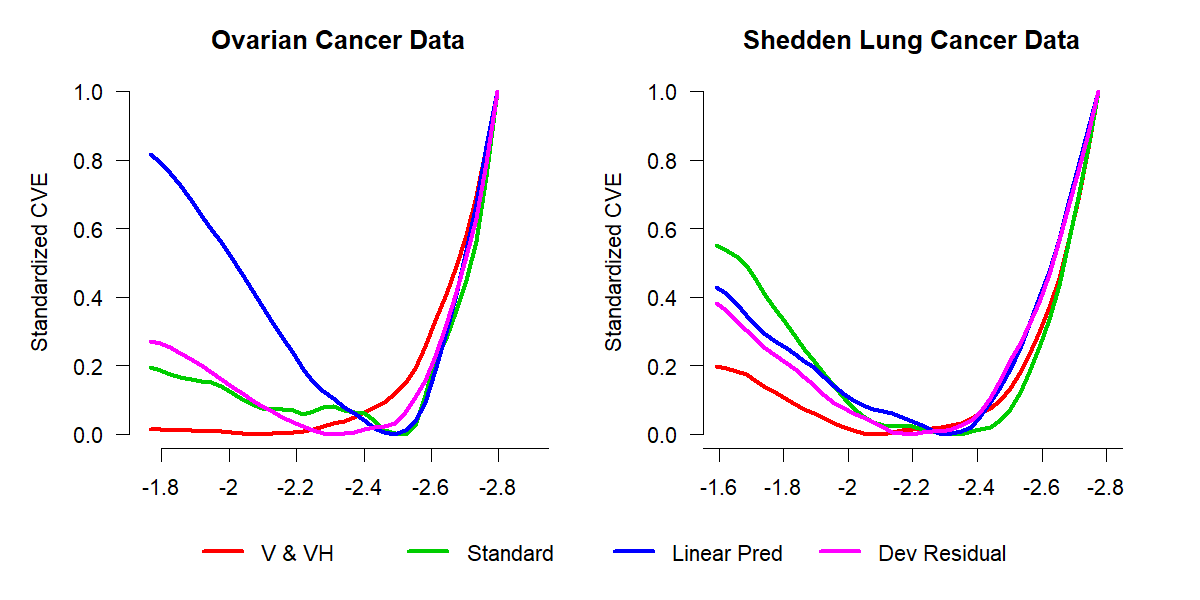
\includegraphics[height= 8cm ]{./figures/figure_5.png}
    \caption{Comparing Cross-Validated Error for Different Methods on Real Data Sets}
\end{figure}	

\par How the CV methods perform on real data reflects what is shown in simulation studies. The standard CVL is the most liberal approach. Deviance Residual and Verweij and Van Houwelingen's CVL approaches were both really conversative, while the standard approach was the second liberal to standard CVL. In Figure 5, the Cross Validated Error is rescaled and plotted for all four methods. A $\lambda$ will be selected when CVE curve reaches its lower point. The blue line, which represents the linear predictor approach, has more curvature near its lowest point. It is easier to pick out the minimum point for this blue curve. Hence this approach is better at picking out signals than the other three approaches. For Verweij and Van Houwelingen's cross-validated partial likelihood, there's almost no signal there.

\section{Discussion}
Four methods of conducting cross-validation for Cox Regression were compared through simulation studies in terms of their predictive accuracy. All cross-validation methods tend to select the more conservative model: with greater value of $\lambda$, and fewer variables selected into the model. Despite of the stability issue, the standard approach is the most liberal one across all scenarios and yield the least MSE. The proposed linear predictor approach performs closely to the standard approach. Under LOOCV, the linear predictor approach out-performs the standardstandard approach. Both Verweij and Van Houwelingen's approach and the proposed Deviance Residual approach perform conservatively, hence not recommended for use in practice. Results from real data application reflects results from the simulation studies.
